\documentclass[journal, a4paper]{IEEEtran}
\usepackage{cite}  
\usepackage{graphicx}
\usepackage{listings}
\usepackage{inconsolata}
\usepackage{subfigure}
\usepackage{url}       
\usepackage{stfloats} 
\usepackage{amsmath}   
\usepackage{array}


\usepackage{Sweave}
\begin{document}
\Sconcordance{concordance:pdf_template3.tex:pdf_template3.Rnw:%
1 10 1 1 40 1 1 1 0 32 1 1 14 54 1 1 17 90 1 1 32 1 6 48 1}


\font\myfont=cmr12 at 18pt
	
	\title{ \myfont Report on 2017 Border Apprehension Statistics}
	\author{Francesco Ignazio Re\\
			Yin Huang	\\
			Yue Emma Wu
			}

	\markboth{Assignment 3 -Section 1 project}{}
	\maketitle

	
	% Each section begins with a \section{title} command
	\section{Introduction}
	% \PARstart{}{} creates a tall first letter for this first paragraph
	
	Apprehensions at the US-Mexico border have declined to near-historic lows over the last few years.
	The objective of this report is to give a deeper insight on this change that has been occuring.
	Through the analysis of the data collected by the U.S. Customs and Border Protection through the years,
	we intend to shed light on the general trend of this phenomenon, focusing on how factors such as time and place have influenced the given outcome.
	
	
	
%	\PARstart{T}{his} section introduces the topic and leads the reader on to the main part.
	
	
	
	
	% Main Part
	\section{Descriptive Data Analysis on sectors and months:}
	
	From 2010 to 2017, the U.S. Customs and Border Protection saw an overall 36 percent decrease in individuals apprehended while trying to enter the country illegally. 






\begin{figure}[!hbt]
\begin{center}

{

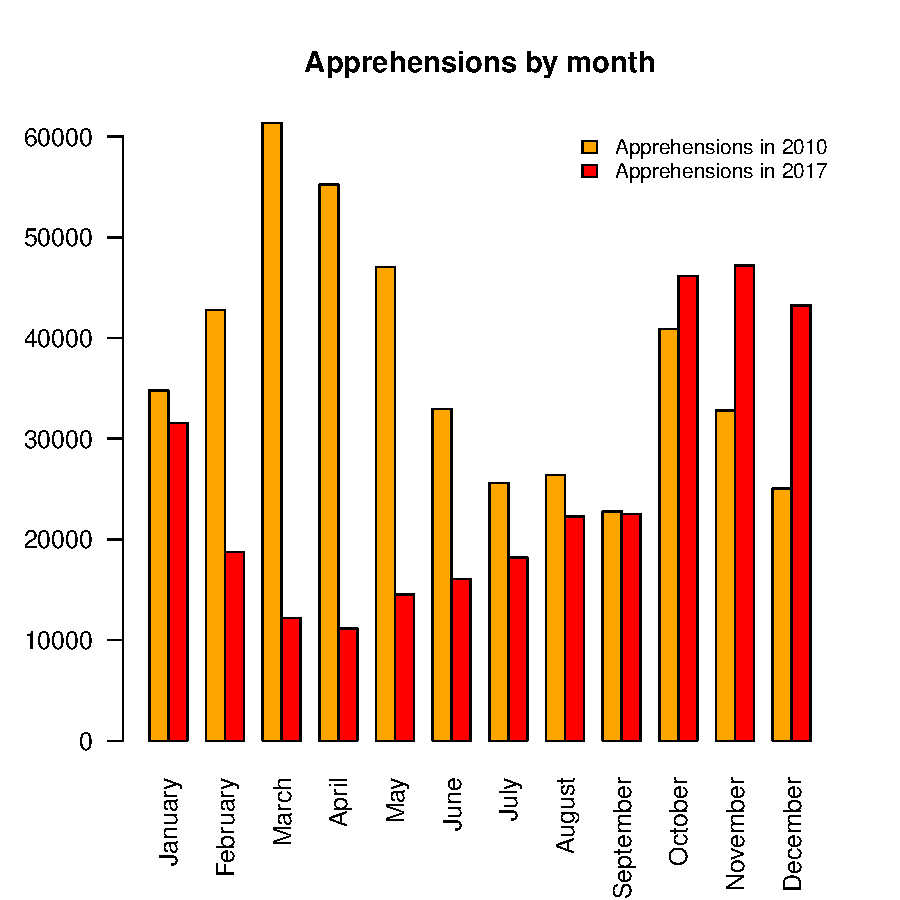
\includegraphics[width=0.4\textwidth]{pdf_template3-fig1}
\caption{Comparing the 2010 and 2017 apprehensions by month}
}

\end{center}
\end{figure} 


	\begin{table}[!hbt]
		% Center the table
		\begin{center}
			% Title of the table
			%\caption{Total Apprehensions}
			\label{tab:simParameters}
			% Table itself: here we have two columns which are centered and have lines to the left, right and in the middle: |c|c|

			
			
			\begin{tabular}{|c|c|}
				% To create a horizontal line, type \hline
				\hline
				% To end a column type &
				% For a linebreak type \\
			Total apprehensions in 2010 & $447731$ \\
				\hline
			 Total apprehensions in 2017 & $286879$ \\
				\hline
			\end{tabular}
		\end{center}
	\end{table}
	
On a first analysis, it's clear the presence of a strong dependence between sectors and months. In other words, different sectors in different months, have a different likelihood of possible observations, as the X-squared test, done on the two sets, shows below.


\begin{enumerate}

\item X-squared test on the 2010 apprehensions by months and sectors.

\subitem X-squared = 9977.5      p-value < 2.2e-16


\item X-squared test on the 2017 apprehensions by months and sectors.

\subitem X-squared = 22656       p-value < 2.2e-16



\end{enumerate}

In both cases, the very small p-value suggests that variables such months and sectors add insigthful information to the analysis.




In fact, we can see that the overall change has actually been characterized by a major drop in certain months and certain places rather than by a constant decline everywhere. By looking at Fig.1, it's easy to see that the most trafficated months in 2010, such as March, April and May are also the ones that have witnessed the greatest decline, figuring the lowest numbers in the data collected in 2017. The cause why this happened may be because of the Trump administration that took office at the very beginning of 2017. Probably, migrants were waiting in those months to see what would happen under Trump before attempting to enter the U.S. illegally.

Visualizing the data by sector, the greatest change has occured in Tuscon, the area with the highest number of apprehensions in the 2010, that observed a drop of over the 80 percent according to the data collected in 2017. 





\begin{figure}[!hbt]
\begin{center}

{

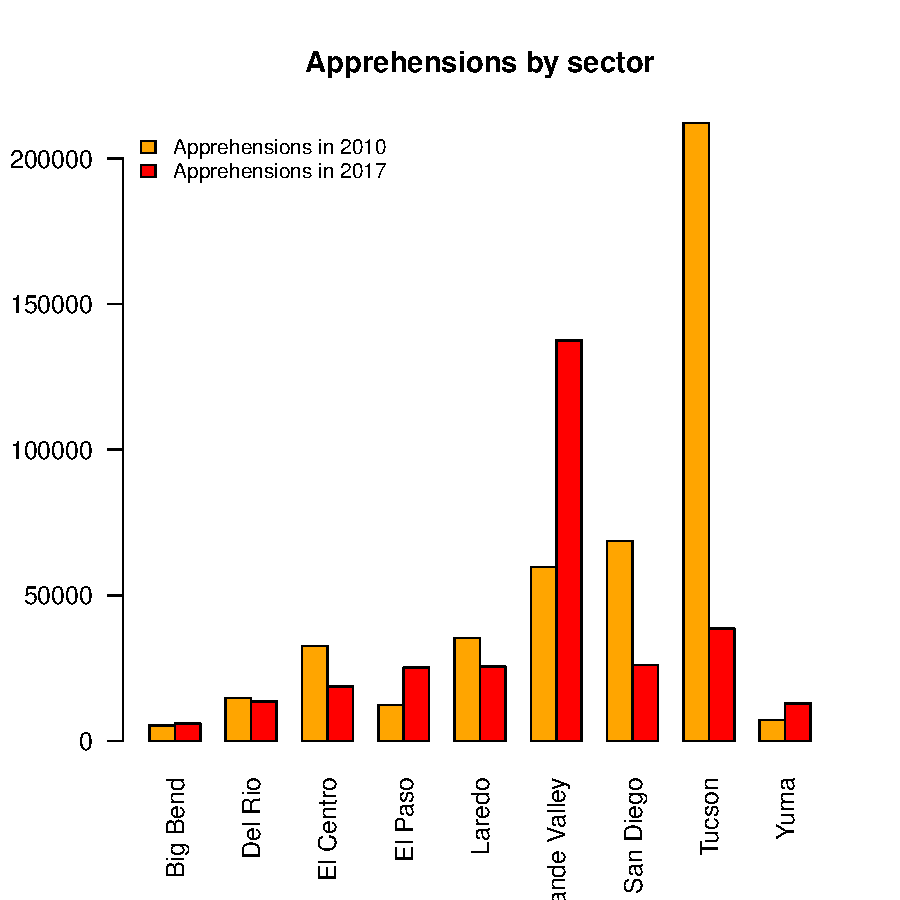
\includegraphics[width=0.4\textwidth]{pdf_template3-fig2}
\caption{Comparing the 2010 and 2017 apprehensions by sector}
}

\end{center}
\end{figure} 

It's interesting to see how some sectors, such as El Paso, Grand Valley and Yuma, have witnessed an increasing in apprehensions. However, this rise is quite uninfluencial when compared with the steep decline had in the sector Tucson. 
Substantiating what just said, here below we compare the change had in the sector Grande Valley, that has a peak in the 2017 apprehensions, with the sector Tucson, that has a peak in the 2010 ones.

\begin{enumerate}

\item T-test on Tucson observations.

\subitem $ H_{o} $ =  true mean of Tuscon's apprehensions in 2010 is the same as in 2017 (alpha = 0.05)

\subitem 95 percent interval = $ (9363.28,  19560.89) $

\subitem mean of the difference = 14462.08 

\subitem p value = $ 6.324e-05 < 0.05$

\item T-test on Grande Valley observations.

\subitem $ H_{o} $ = true mean of RGV's apprehensions in 2010 is the same as in 2017 (alpha = 0.05)

\subitem 95 percent interval = $ (-12283.0782   -682.9218) $

\subitem mean of the difference = $ -6483  $

\subitem p value = $  0.03167 < 0.05$

\end{enumerate}

The above test highlights the difference between the two sectors, showing that the Tuscon sector played a critical role in the change of apprehensions between the two years whereas in the second case the p-value is much bigger.

The apprehensions sorted by months show a similar pattern. Let's compute the t-tests for the three most trafficated months in both the years.

\begin{enumerate}

\item  T-test on the three most trafficated months in 2010: March, April, May.

\subitem $ H_{o} $ = mean of the difference between the observations in March, April, May in 2010  and in 2017.

\subitem 95\% interval = $ (20742.45, 63125.55) $

\subitem mean of the difference = $  41934  $

\subitem p value = $ 0.01352 < 0.05$


We can reject the null hypothesis. March - May 2010 means are significantly different from those in 2017, with 95\% confidence. 

\item  T-test on the three most trafficated months in 2017:  October, November and December.

\subitem $ H_{o} $ = mean of the difference between the observations in October, November and December in 2010  and in 2017.

\subitem 95\% interval = $ (-29127.621,  3856.288) $

\subitem mean of the difference = $ -12635.67  $

\subitem p value = $ 0.081 $


We cannot reject the null hypothesis. October - December 2017 means are not significantly different from those in 2010. 

\end{enumerate}






	\section{Analysis on the trend over 17 years}


As another way to analyze the trend, we try to get some insight looking at the monthly apprehensions spanned along a period of seventeen years, from 2000 to 2017. 
What we can work out, as highlighted in Fig. 3, is that there are months that have witnessed a consistent change in apprehensions during the years (January, February, March, April), while others tended to stick up around a more limited range of values such as October, November, December. Moreover, the first months of the year seem to have been the most trafficated ones over all. 



\begin{figure}[!hbt]
\begin{center}

{

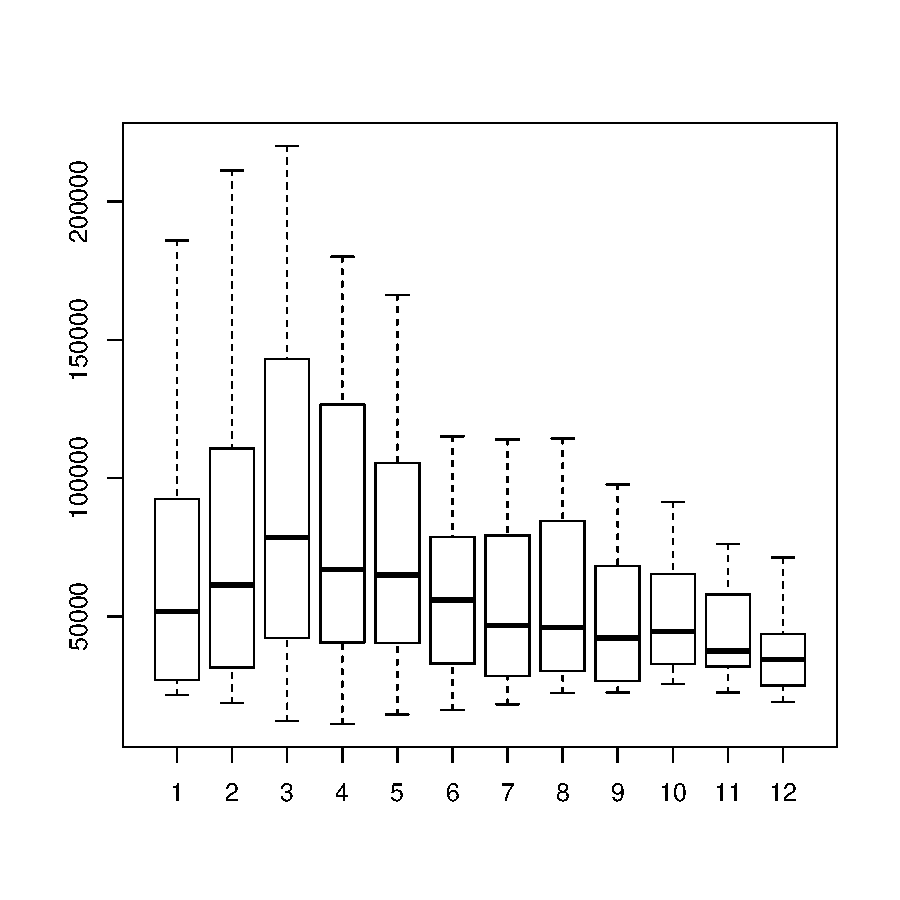
\includegraphics[width=0.4\textwidth]{pdf_template3-fig4}
\caption{Time series of Apprehension from 2000 to 2017}
}

\end{center}
\end{figure} 

Through Fig.4, we can see that from 2000, there's been a steady decrease in apprehensions, reaching its lowest value in  the first months of 2017. Overall, the apprehensions plummeted by approximately 80\%, from a high of over 1.6 million in 2000 to around 300,000 in 2017.A possible cause of this trend may lay on the administrative decisions taken over the years that may have deceived people from crossing the border illegaly. 

\begin{figure}[!hbt]
\begin{center}

{

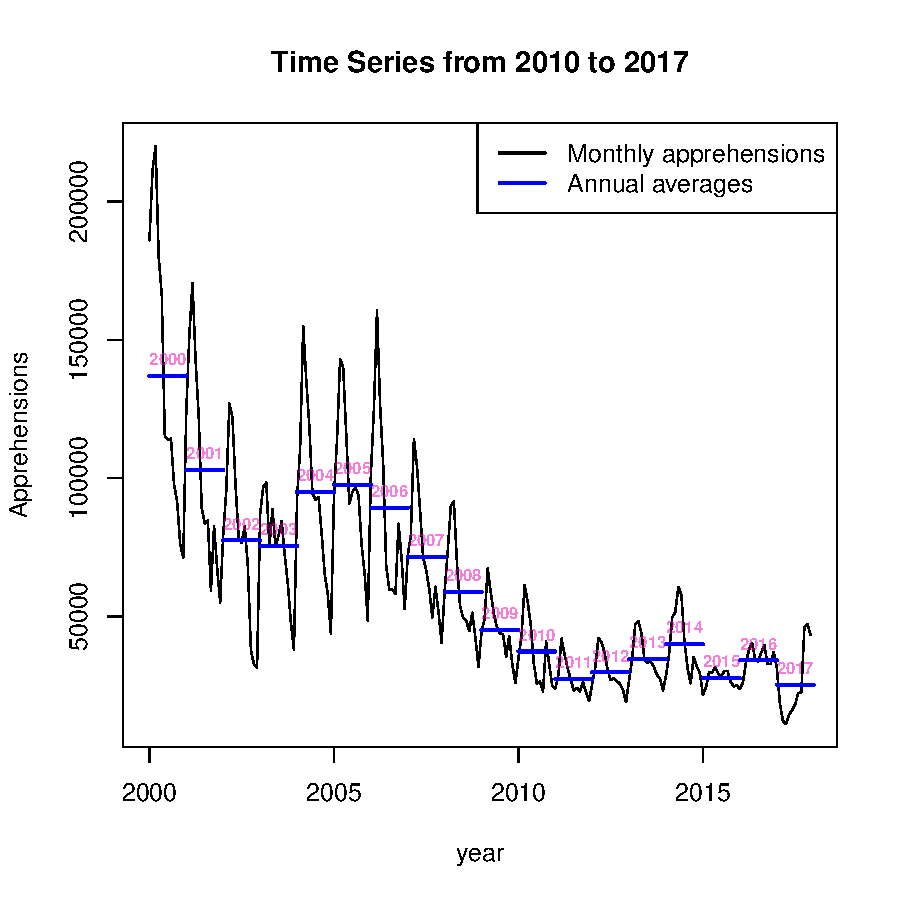
\includegraphics[width=0.5\textwidth]{pdf_template3-fig3}
\caption{Time series of Apprehension from 2000 to 2017}
}

\end{center}
\end{figure} 


	\begin{thebibliography}{5}
		
		
		
  	\bibitem{1} All the result of the above tests are documented in the document R-code-project.R
	
		\bibitem{2}
     \url{https://www.cnn.com/2017/05/09/politics/border-crossings-apprehensions-down-trump/index.html}
		
	\end{thebibliography}
		
	

\end{document}
